\chapter{Use Case Analysis : Problem 5}
\vspace{8pt}

\section{Use Cases List}

\begin{flushleft}

\vspace{5pt}
\noindent
1)	Calculate regular number: user switch on calculator, the regular number calculation mode starts by default.
\vspace{4pt}
\leavevmode\\
\noindent
2)	Input regular number: user types intended number and operators
\vspace{4pt}
\leavevmode\\
\noindent
3)	Recall last 10 results: user recollects historical 10 calculation results
\vspace{4pt}
\leavevmode\\
\noindent
4)	Calculate special number: the special number calculation mode starts by default.
\vspace{4pt}
\leavevmode\\
\noindent
5)	Get PI: user gets approximate number of PI directly
\vspace{4pt}
\leavevmode\\
\noindent
6)	Calculate circular area: user gets approximate circular area result regarding input radius using PI
\vspace{4pt}
\leavevmode\\
\noindent
7)	Calculate circular circumference: user gets approximate circular circumference regarding input radius using PI
\vspace{4pt}
\leavevmode\\
\noindent
8)	Input radius value: user type numerical value of radius for a targeted circular
\leavevmode\\

\end{flushleft}

\section{Use Cases Diagram & Description}

\begin{figure}[H]
\centering  %图片全局居中
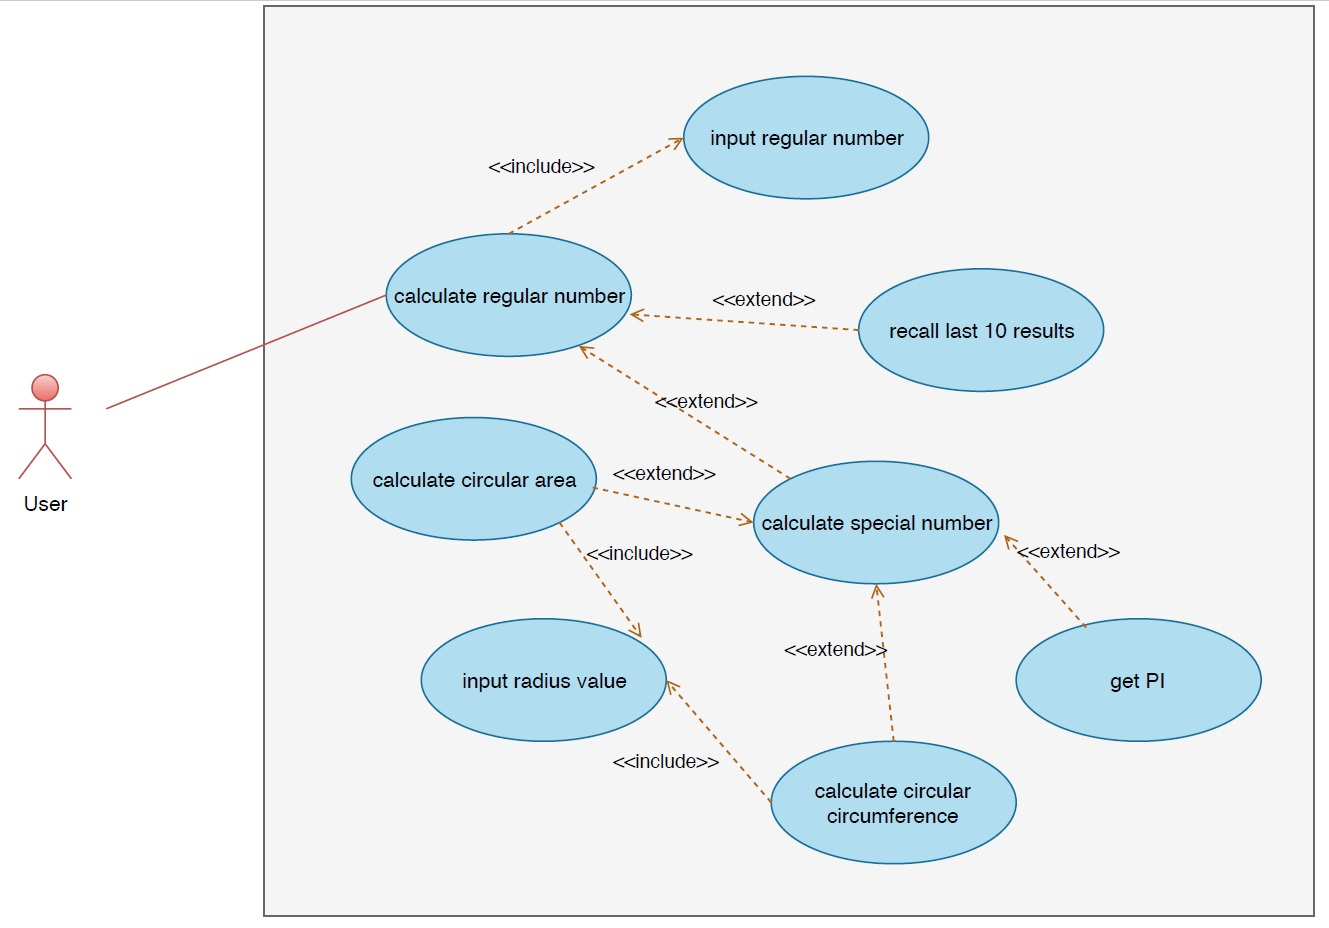
\includegraphics[width=0.9\textwidth]{images/use_case_for_all.jpg}
\caption{Use Case Diagram}
\end{figure}


\begin{figure}[H]
\centering  %图片全局居中
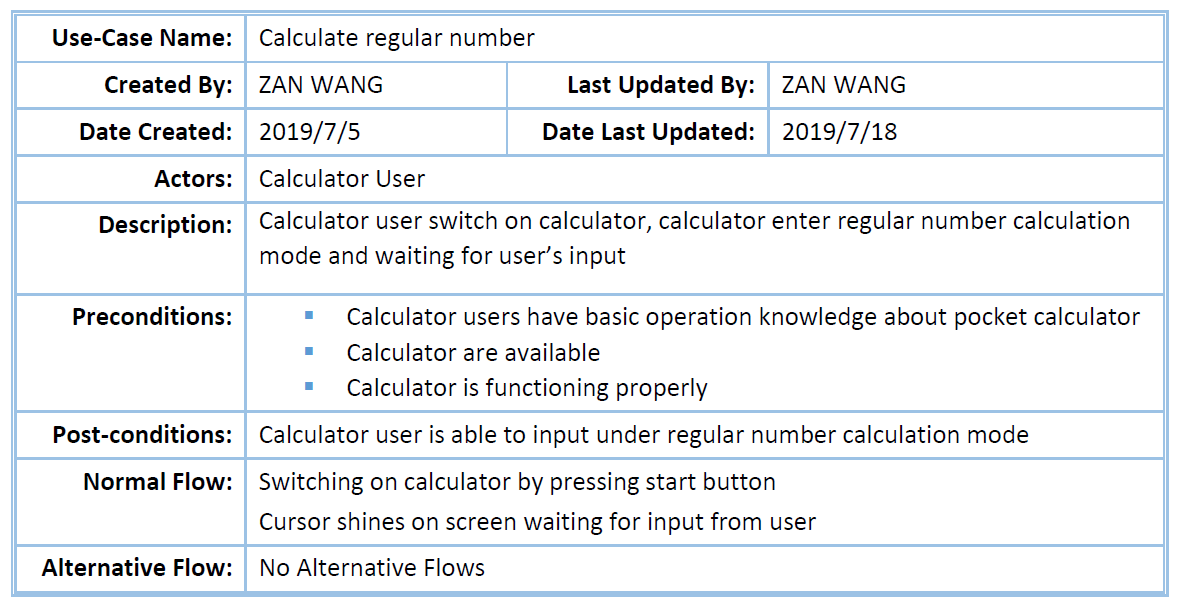
\includegraphics[width=0.9\textwidth]{images/use_case/UC_crn.PNG}
\end{figure}

\begin{figure}[H]
\centering  %图片全局居中
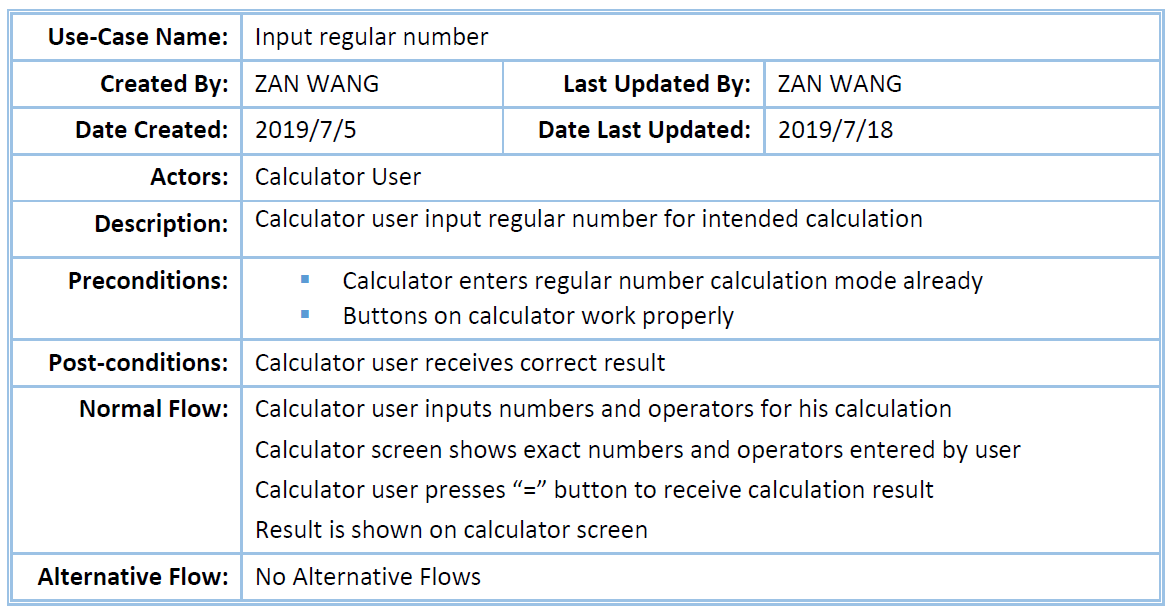
\includegraphics[width=0.9\textwidth]{images/use_case/UC_irn.PNG}
\end{figure}


\begin{figure}[H]
\centering  %图片全局居中
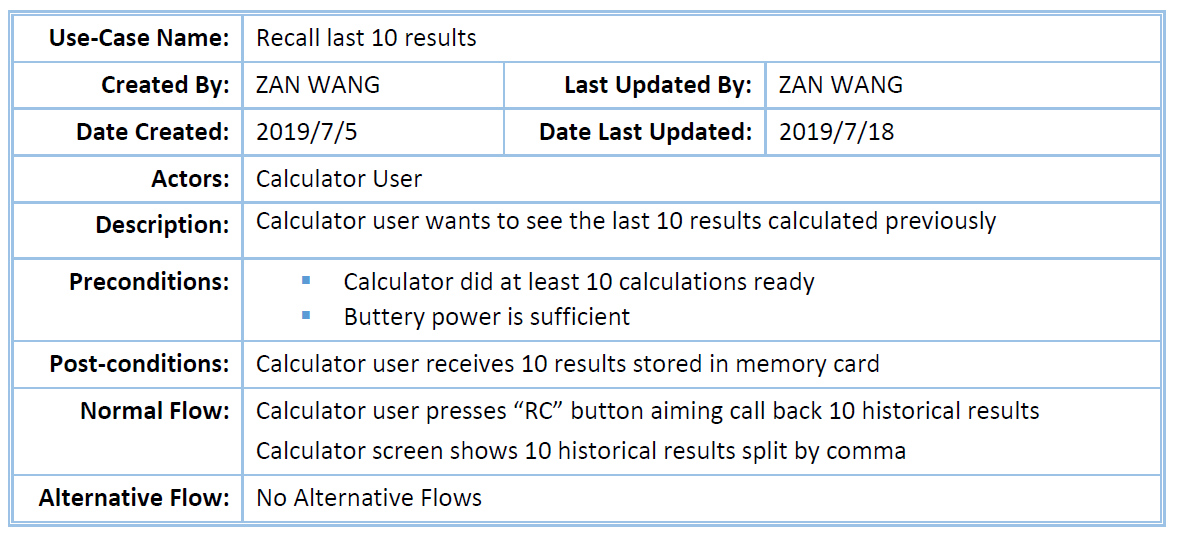
\includegraphics[width=0.9\textwidth]{images/use_case/UC_rl10r.PNG}
\end{figure}

\begin{figure}[H]
\centering  %图片全局居中
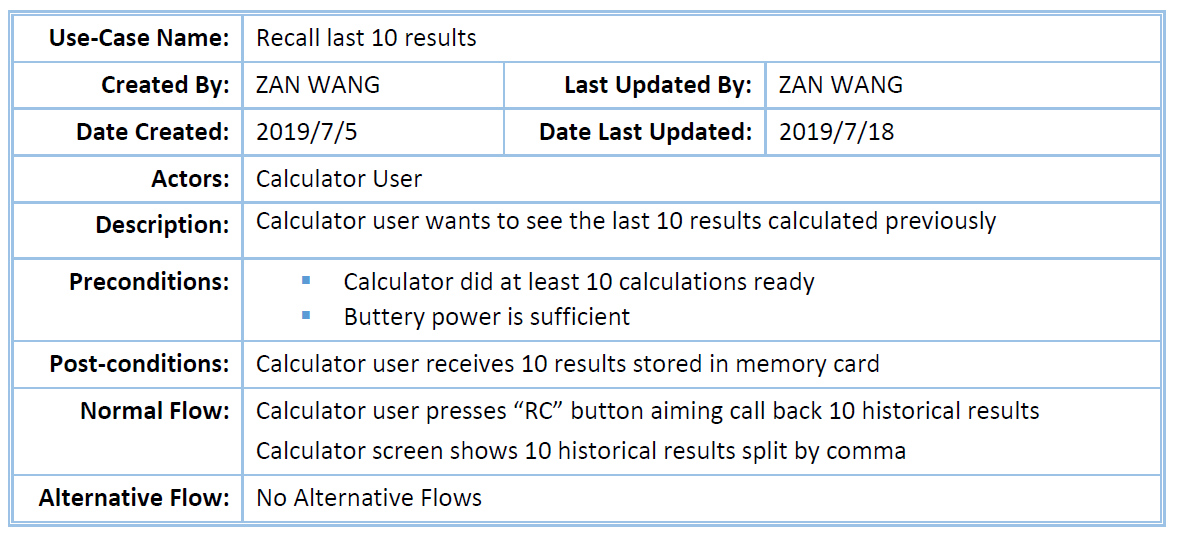
\includegraphics[width=0.9\textwidth]{images/use_case/UC_rl10r.PNG}
\end{figure}

\begin{figure}[H]
\centering  %图片全局居中
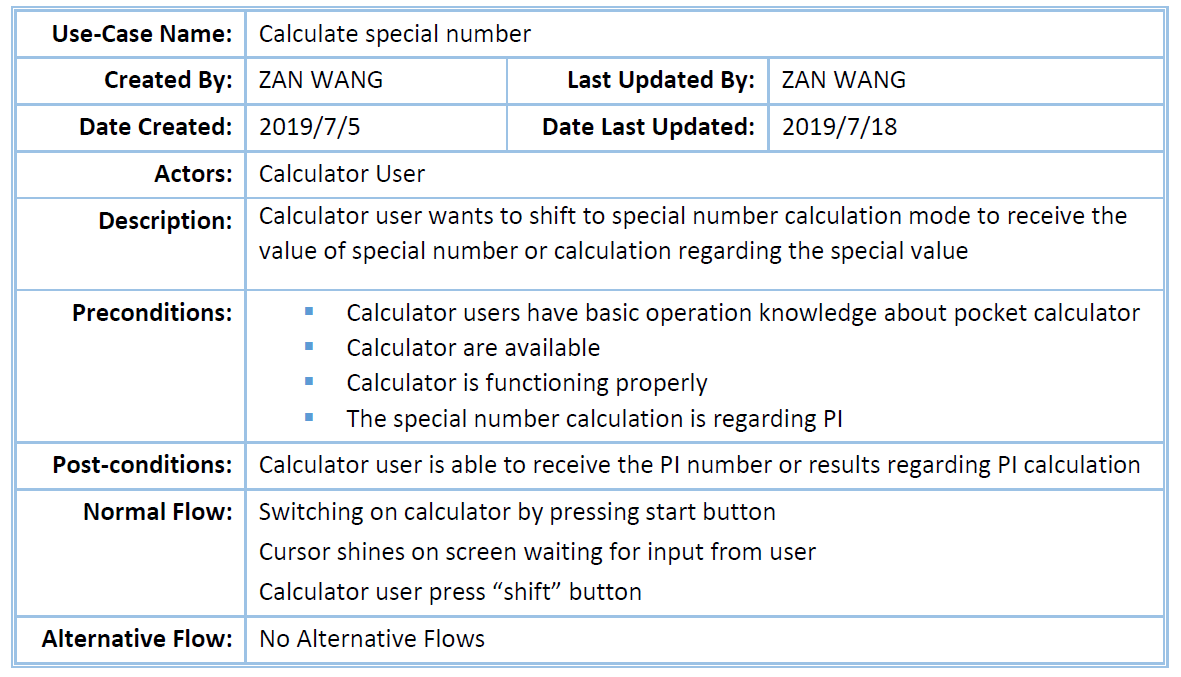
\includegraphics[width=0.9\textwidth]{images/use_case/UC_csn.PNG}
\end{figure}

\begin{figure}[H]
\centering  %图片全局居中
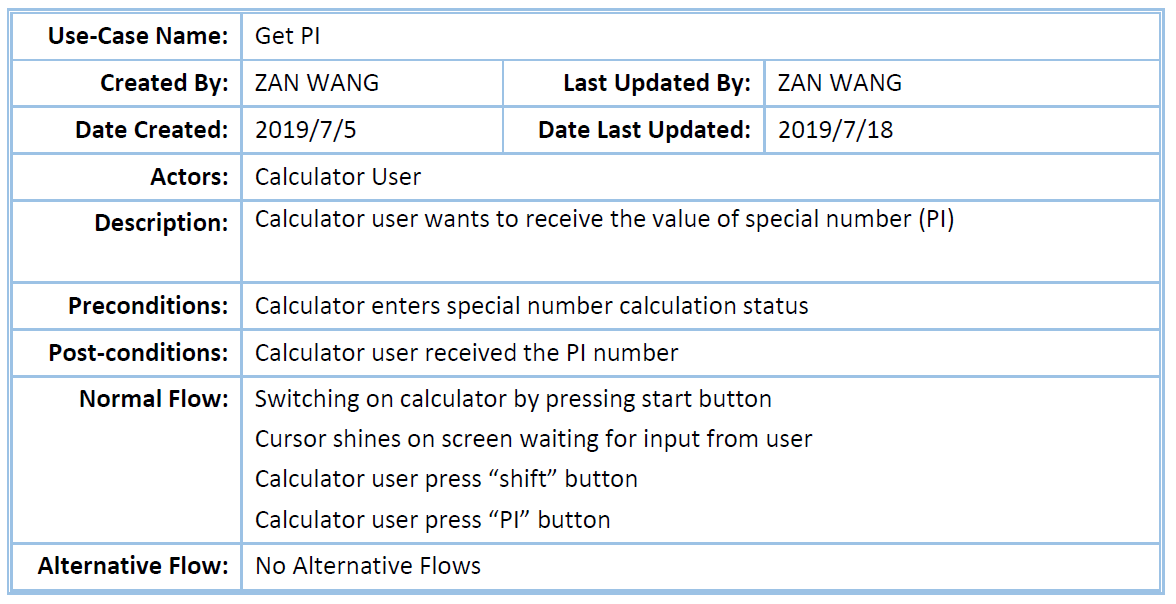
\includegraphics[width=0.9\textwidth]{images/use_case/UC_get_pi.PNG}
\end{figure}


\begin{figure}[H]
\centering  %图片全局居中
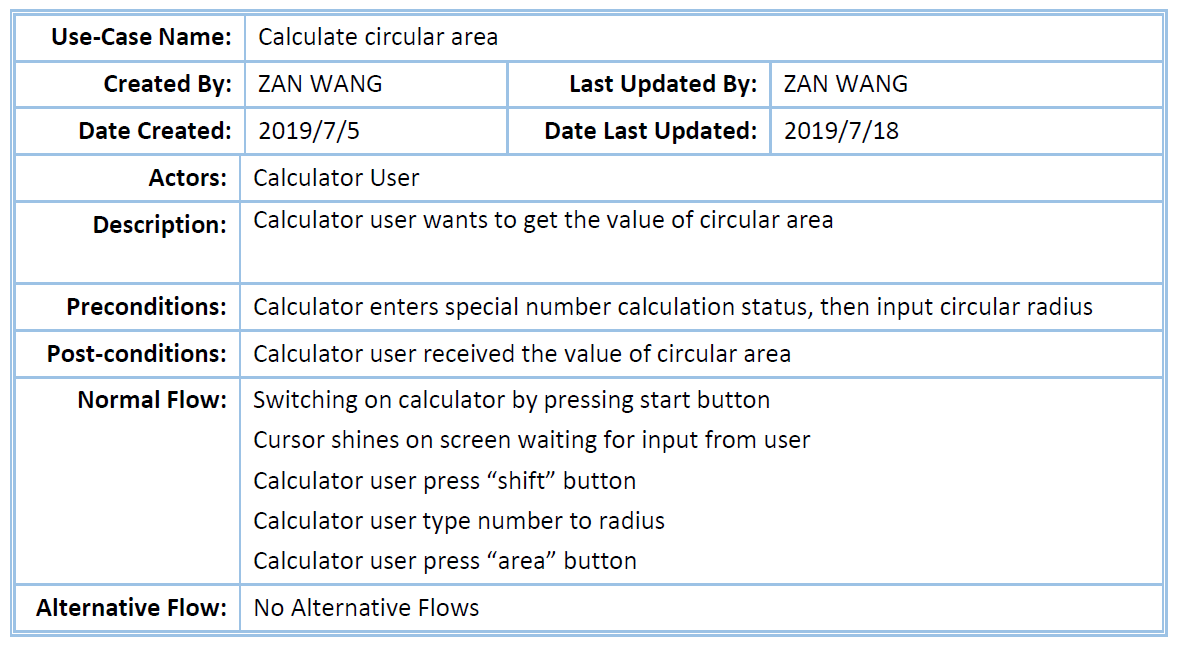
\includegraphics[width=0.9\textwidth]{images/use_case/UC_cca.PNG}
\end{figure}

\begin{figure}[H]
\centering  %图片全局居中
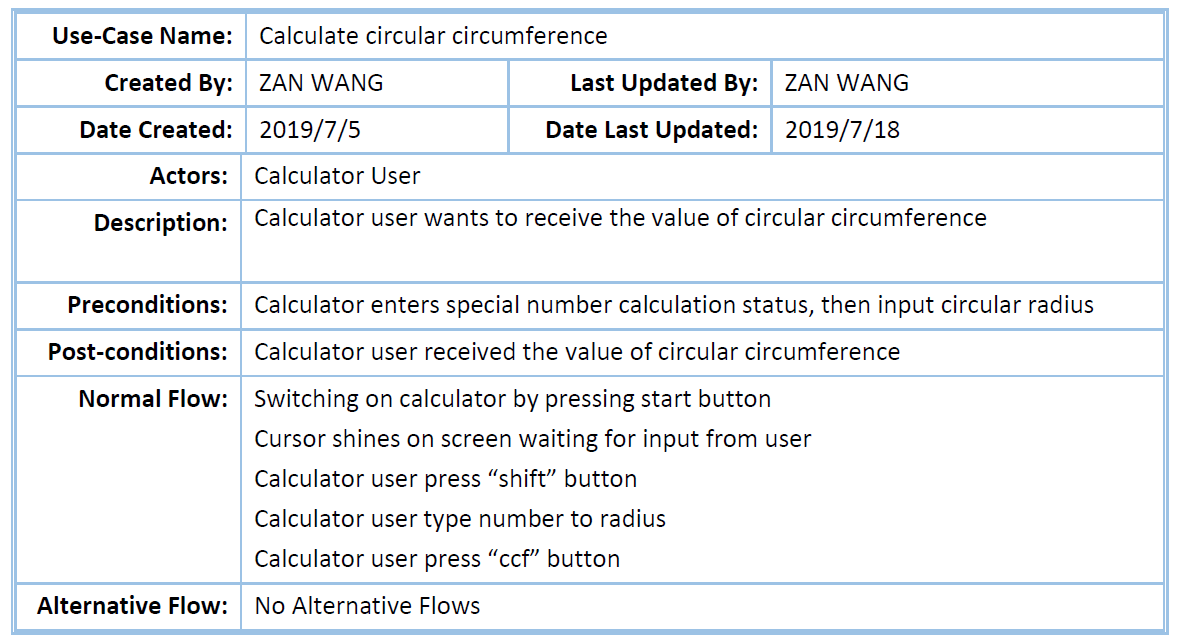
\includegraphics[width=0.9\textwidth]{images/use_case/UC_ccc.PNG}
\end{figure}

\begin{figure}[H]
\centering  %图片全局居中
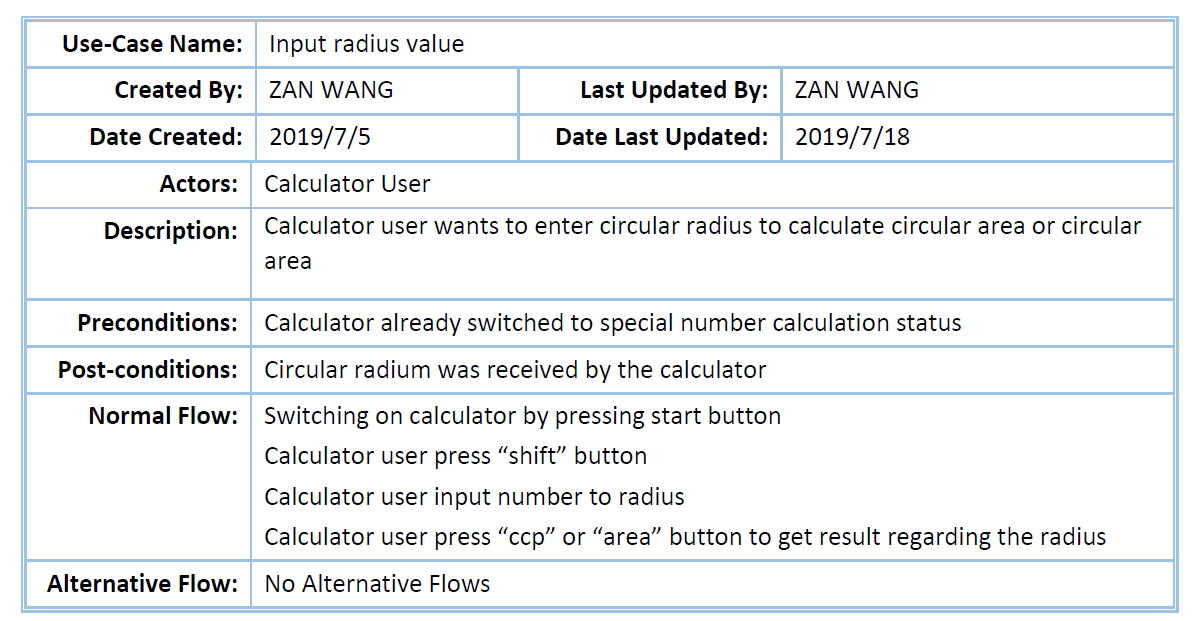
\includegraphics[width=0.915\textwidth]{images/use_case/UC_irv.PNG}
\end{figure}

\begin{figure}[H]
\centering  %图片全局居中
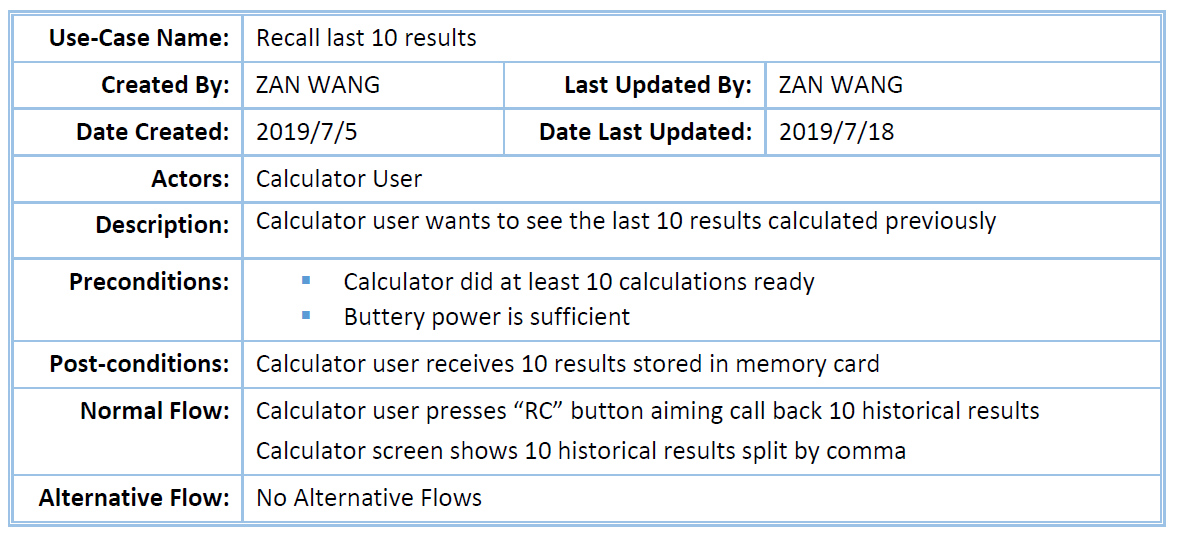
\includegraphics[width=0.9\textwidth]{images/use_case/UC_rl10r.PNG}
\end{figure}



\section{Sequence Diagram for Main Use Cases}

\begin{figure}[H]
\centering  %图片全局居中
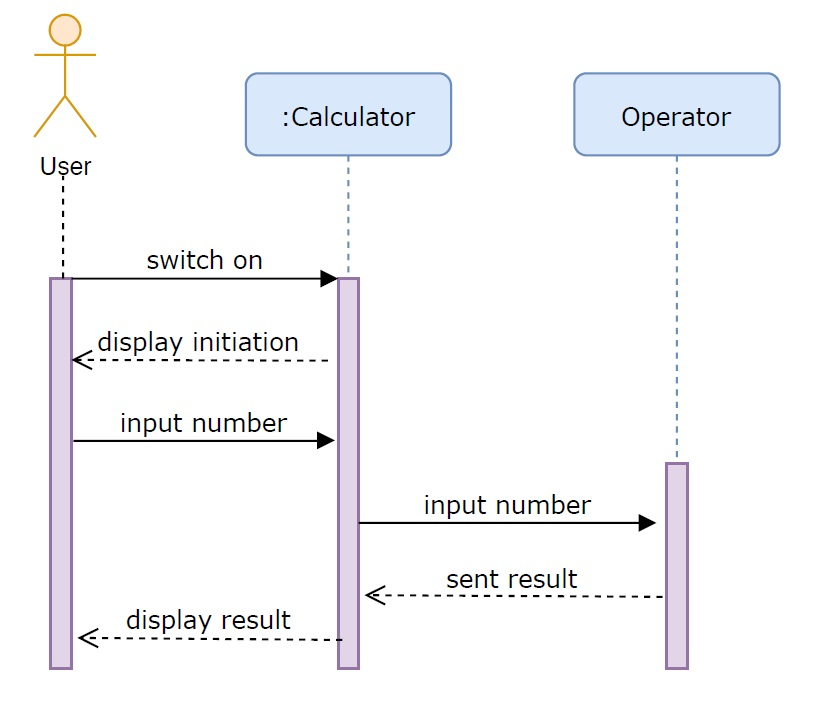
\includegraphics[width=0.6\textwidth]{images/SD/ccn.jpg}
\caption{Input Regular Number}
\end{figure}

\begin{figure}[H]
\centering  %图片全局居中
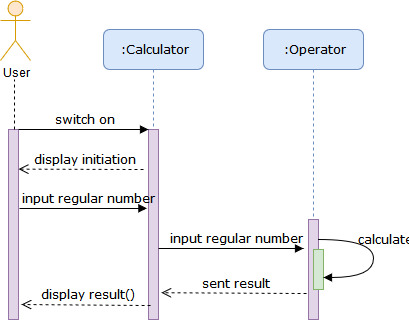
\includegraphics[width=0.6\textwidth]{images/SD/irn.jpg}
\caption{Calculate Regular Number}
\end{figure}

\begin{figure}[H]
\centering  %图片全局居中
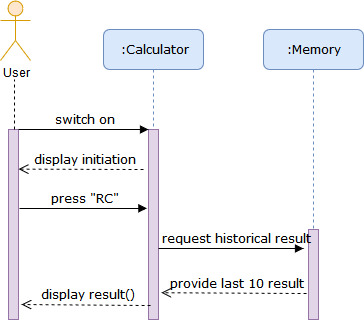
\includegraphics[width=0.6\textwidth]{images/SD/rl10r.jpg}
\caption{Recollect Historical Result}
\end{figure}

\begin{figure}[H]
\centering  %图片全局居中
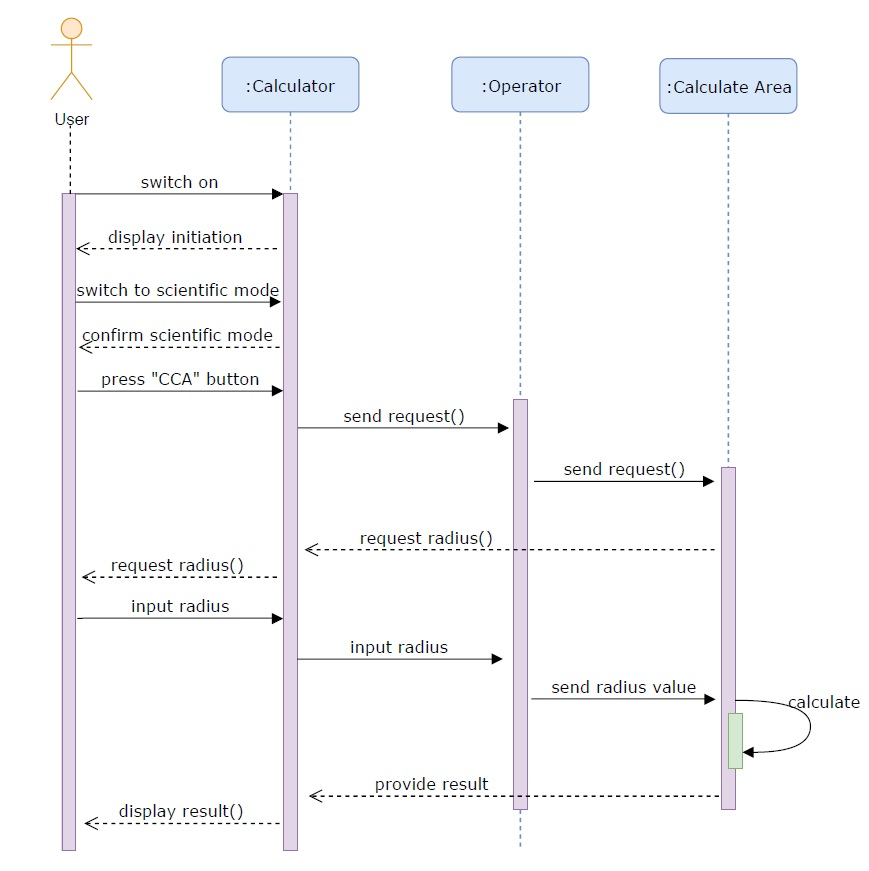
\includegraphics[width=0.7\textwidth]{images/SD/cca.jpg}
\caption{Calculate Circular Area}
\end{figure}

\begin{figure}[H]
\centering  %图片全局居中
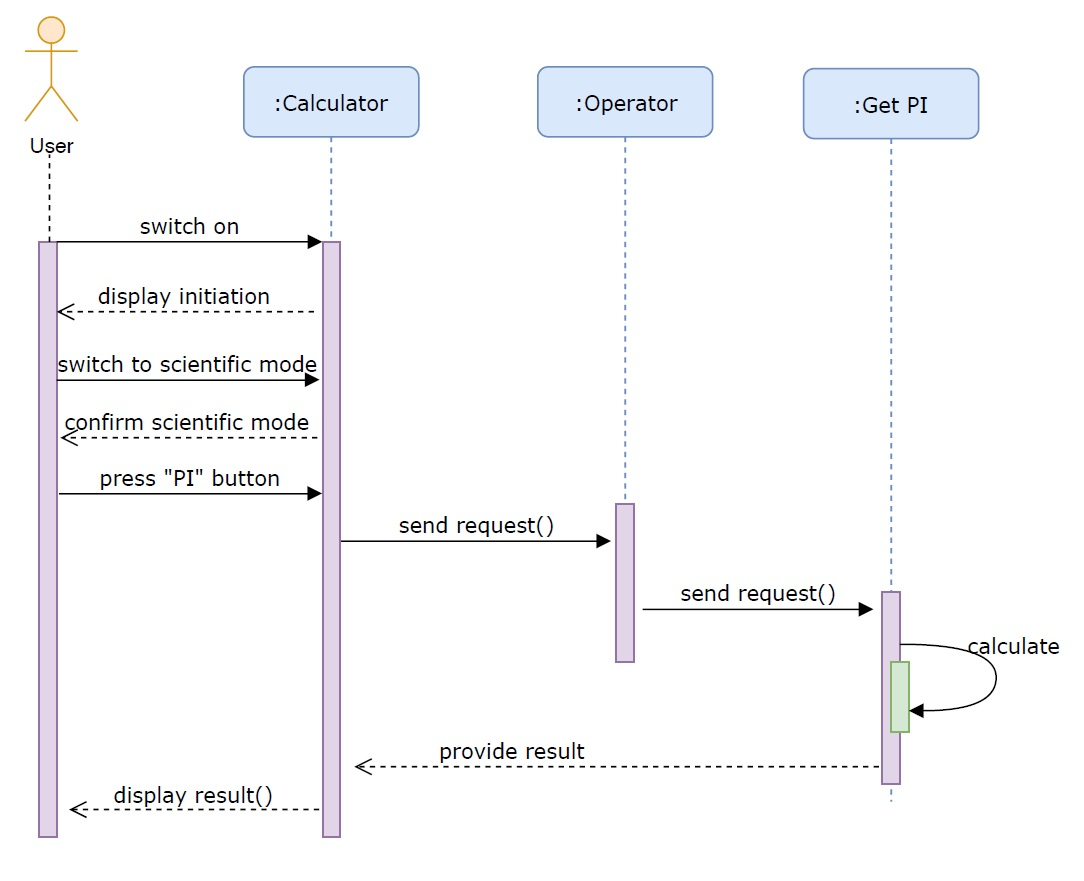
\includegraphics[width=0.6\textwidth]{images/SD/getpi.jpg}
\caption{Calculate PI}
\end{figure}

\begin{figure}[H]
\centering  %图片全局居中
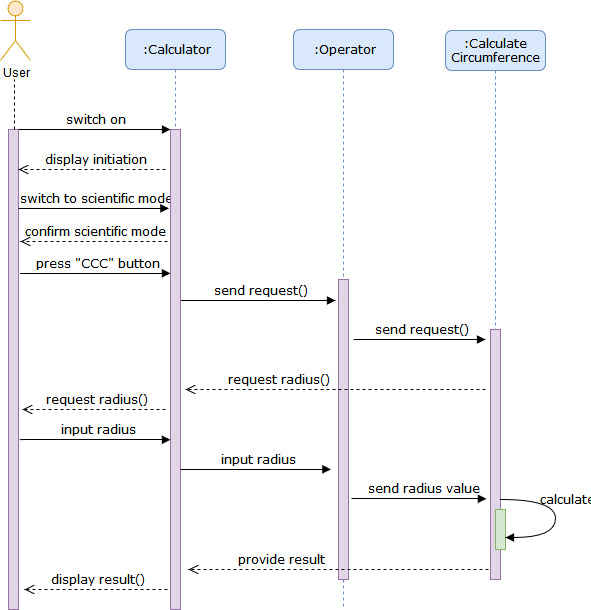
\includegraphics[width=0.6\textwidth]{images/SD/ccc.jpg}
\caption{Calculate Circular Circumference}
\end{figure}



\vspace{50pt}
\section{Activity Diagram}

\begin{flushleft}
\vspace{8pt}
\noindent
Activity Diagrams describe how activities are coordinated to provide a calculation results which can be at different levels of abstraction. Typically, user needs to switch on the calculator first, then the user could choose to trace the last 10 results, calculate regular number, or calculate special scientific number (PI). If user want to have scientific number, then functions related to this scientific number could be applied. Taking PI as an example, addition to get the PI value, user also can know circular area and circular circumference after inputting exact radius value for intended circular.
\end{flushleft}


\begin{figure}[H]
\centering  %图片全局居中
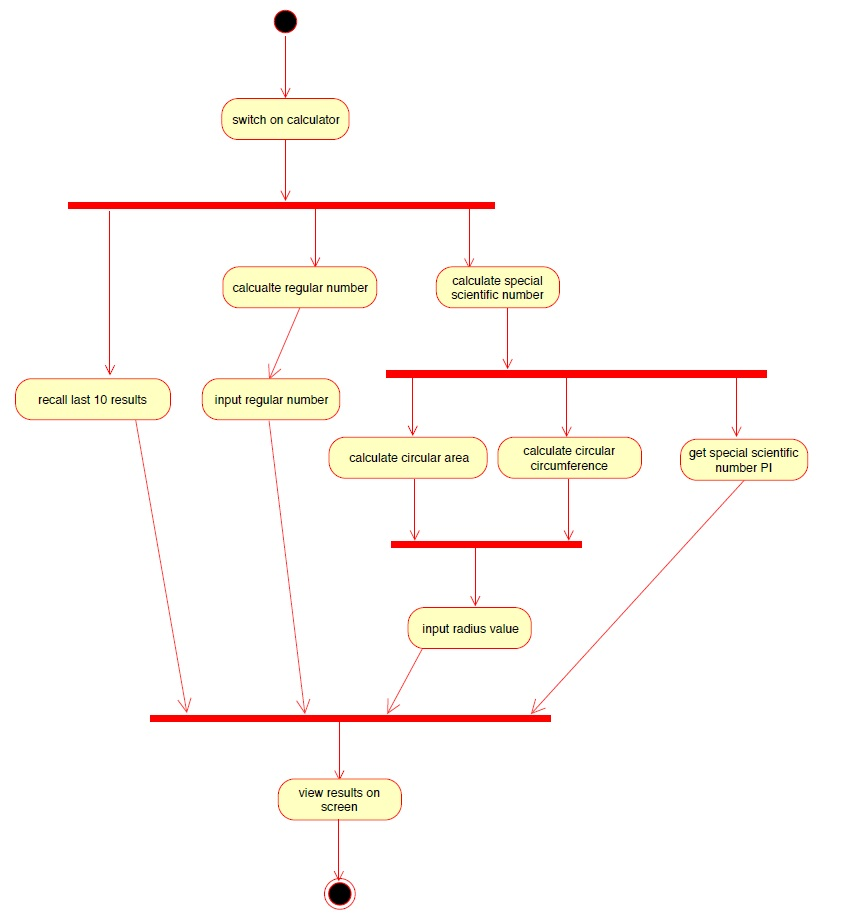
\includegraphics[width=0.8\textwidth]{images/activity_diagram.jpg}
\caption{Activity Diagram}
\end{figure}



